\documentclass[etudiants]{support-iutrs}
\usepackage{pdfpages}
\usepackage{wrapfig}
\usepackage{graphicx}
\usepackage{subfig}

\infos{Benedick Steve, Meyblum Jean, Hagner Kevin}{P31}{T306AMAO}

\sujet{}
\titre{Ergonomie dans notre projet T3}

\begin{document}
\header
\section{Petite introduction sur notre projet}

Notre projet a pour but la gestion informatique des emprunts et achats de bandes dessinées (\emph{BD}) réalisés par un particulier.
Afin de gérer la saisie et l’enregistrement des bandes dessinées nous allons modifier une application déjà existante : \emph{Royal}. 
Dans le but de faciliter l'ajout de \emph{BDs} dans Royal nous allons aussi mettre en place une application pour les téléphones Android : \emph{Royal\_Scanner}.
Cette application permettra de scanner les codes barres afin de les envoyer au client PC Royal via un email.

Pour analyser l'ergonomie dans notre projet T3 nous travaillerons dans deux parties distinctes: 

--- La première traitera de l'ergonomie dans \emph{Royal}.

--- La seconde traitera, elle, de l'ergonomie dans \emph{Royal\_Scanner}.

\section{Ergonomie dans Royal}
Dans cette partie nous détaillerons l'interface graphique de la page principale de \emph{Royal} mais les mêmes propriétés sont appliquées aux autres pages de l'application. 

\subsection{Agencement de la fenêtre}
L'agencement de l'application respecte assez bien les critères d'agencement vu en cour.

\begin{wrapfigure}[5]{l}[1cm]{5cm}
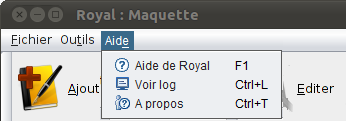
\includegraphics[width=5cm]{img/app_pc_maquette_menu.png}
\end{wrapfigure}

Tout d'abord nous retrouvons un menu regroupant les actions secondaires de l'application tels que les préférences ou encore l'aide de Royal. 
Ce menu n'est pas surchargé (au maximum trois choix possibles), et rappel pour chaque action des raccourcis clavier associés (ceux-ci améliorent grandement la vitesse d'utitilisation du programme).

\begin{wrapfigure}[6]{r}[1cm]{8cm}
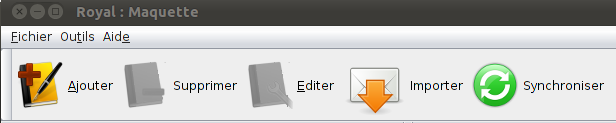
\includegraphics[width=8cm]{img/app_pc_maquette_btn.png}
\end{wrapfigure}

En dessous, nous retrouvons 5 boutons permettant d'effectuer les 5 principales actions de l'application. 
Ces 5 boutons sont accompagnés d’icônes, ce qui les rends plus visible et facilite leurs compréhensions.
Ils sont placés à un endroit ou ils sont très visible et facile d'accès ce qui est important vu qu'il s'agit des principales fonctionnalités de notre applications.

Dans la partie centrale de l'application, nous retrouvons deux parties :

\begin{wrapfigure}[13]{l}[1cm]{7.5cm}
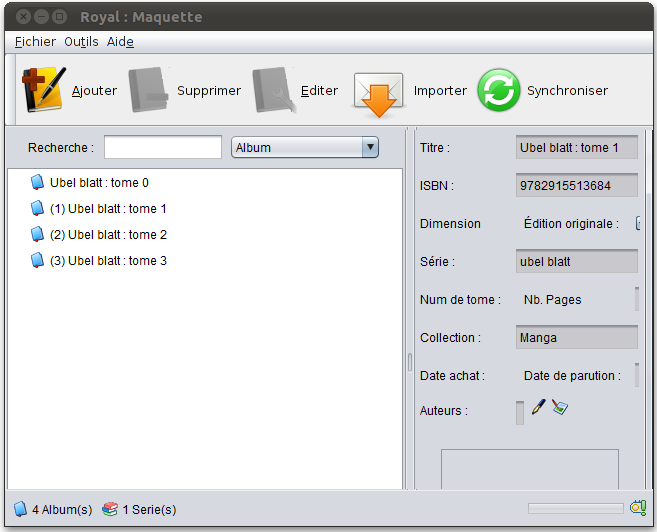
\includegraphics[width=7.7cm]{img/app_pc_maquette2.png}
\end{wrapfigure}
- \textbf{À gauche}: la partie affichant les différents albums enregistrés dans \emph{Royal} en fonction du critère d'affichage sélectionné. 

- \textbf{À droite}: la partie affichant les différentes informations sur l'album sélectionné.

Un problème d'ergonomie dans la partie gauche peu être observé lorsque la fenêtre est trop petite car certaines informations n'ont pas la place pour être affichées. 
Mais le problème disparaît une fois la fenêtre agrandie. 
Pour corriger ce problème nous pouvons définir une largeur de fenêtre minimale afin d'assurer l’affichage de toute les informations. 

\begin{wrapfigure}[5]{r}[1cm]{6cm}
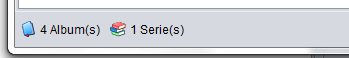
\includegraphics[width=6cm]{img/app_pc_maquette_bas.png}
\end{wrapfigure}

Enfin dans le bas de page nous retrouvons un récapitulatif du nombre d'albums et de séries présents dans l'application.
Cette information étant optionnelle, ce n'est pas grave si elle est placée en-bas dans la fenêtre.

\subsection{Couleurs et polices}
Les couleurs ainsi que les polices choisies dans l'application \emph{Royal} respectent assez bien les critères vu en cours.

L'application utilise des couleurs neutres et un fond claire. 
La partie regroupant les 5 boutons a un fond utilisant un autre gris que celui utilisé en fond de l'application, se qui permet de la distinguer rapidement. 
\begin{wrapfigure}[5]{l}[1cm]{6cm}
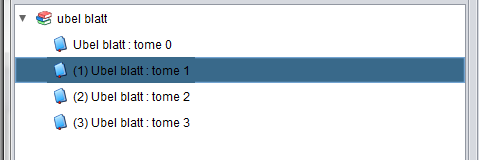
\includegraphics[width=6cm]{img/app_pc_maquette_elmt_selec.png}
\end{wrapfigure}

La partie listant les albums à aussi un fond blanc. Ce qui, à nouveau, permet de distinguer facilement cette partie du reste. 
De même, l'élément sélectionné aura un fond bleu, ce qui provoque un contraste suffisamment fort pour qu'il soit très bien repéré parmi tout les autres.  

Pour le texte dans l'application, une seul police est utilisée. 
Cela nous permet de garder une homogénéité et d'éviter de perdre le lecteur dans un code de police ambigus.
De même une seule couleur est utilisée : le noir, car il contraste bien avec les fond clairs utilisés.  

\section{Critères ergonomiques}
\subsection{Compatibilité} 

\begin{wrapfigure}[5]{r}[1cm]{8cm}
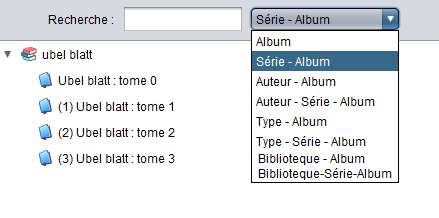
\includegraphics[width=8cm]{img/app_pc_maquette_lst.png}
\end{wrapfigure}\subparagraph{}
Afin d'assurer cette compatibilité, différents types d'affichages de la liste des albums seront proposé à l'utilisateur.
Ces différents types d'affichage se feront en fonctions de critères, tels que l'auteur, le type ou encore la bibliothèque.


\subsection{Guidage et traitements des erreurs} 
Afin de faciliter l'utilisation, l'utilisateur doit être guidé lors de l'utilisation du logiciel.

\subsubsection{Dans la partie ajout/édition d'un album:}

\begin{wrapfigure}[5]{l}[1cm]{8cm}
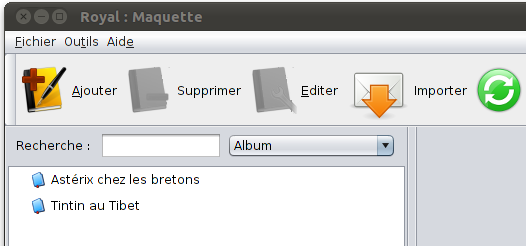
\includegraphics[width=8cm]{img/app_pc_maquette_btn_grise.png}
\end{wrapfigure}\subparagraph{}

Tout d'abord, les boutons des actions ne pouvant être effectués sont grisé (par exemple la suppression ou l’édition d'un album lorsque aucun album n'est sélectionné).
\clearpage

\begin{figure}[h!]
\begin{center}
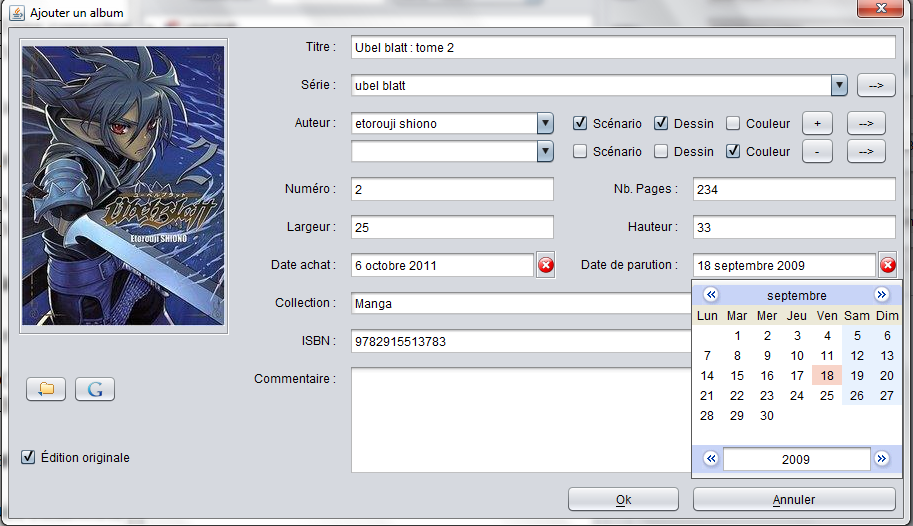
\includegraphics[width=12cm]{img/app_pc_maquette_ajout_album.png}
\end{center}
\end{figure}
Lors de l'ajout de date un calendrier est proposé à l'utilisateur afin qu’il sélectionne une date (ce mode de saisi d'une date permet aussi de limiter les erreurs).

Lors de l'ajout d'auteurs, des \emph{radios button} sont mis en place afin de permettre à l'utilisateur de choisir la fonction de l'auteur (tels que le dessin, le scénario...)

Pour éviter à l'utilisateur de saisir plusieurs fois la même information (par exemple l'auteur) il sera possible d'afficher une liste proposant les divers séries, auteurs, collections et bibliothèques déjà saisies dans l'application.

De même, pour éviter le surplus de champs dans la fenêtre, des boutons on été mis en place pour permettre d'ajouter plus d'informations sur un élément (bouton ->) ou répéter un élément (bouton + pour les auteurs).

\begin{figure}[h!]
\begin{center}
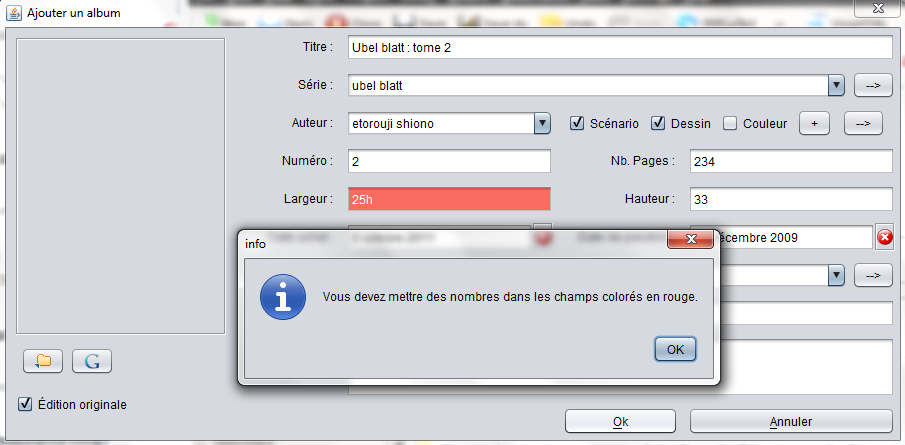
\includegraphics[width=12cm]{img/app_pc_maquette_erreur.png}
\end{center}
\end{figure}

Des vérifications sur la validité des informations ajoutés dans les champs numérique tels que le numéro de tome on été ajoutés. 
En cas de mauvaise saisie un message d'erreur apparaît afin d'inviter l'utilisateur à ressaisir l'information dans le bon format.
Les champs comportant des erreurs sont colorés en rouge, ce qui permet d'être facilement trouvés par l'utilisateur. 

Une vérification sur la validité de l'\emph{ISBN} sera mis en place pour vérifier que celui-ci soit d'un bon format (\emph{ISBN 10} ou \emph{ISBN 13}).

De même le format utilisé (cm) devra être ajouter à la fin de l'écriture de la longueur et la largeur afin d'éviter toute confusion avec d'autres formats.    
\clearpage

\subsection{Partie importation albums}

\begin{wrapfigure}[12]{r}[1cm]{5cm}
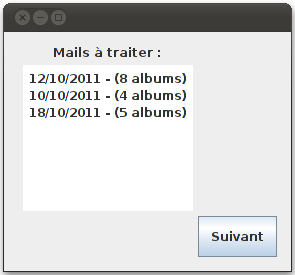
\includegraphics[width=5cm]{img/import_mail.png}
\end{wrapfigure}\subparagraph{}

Lors de l'importation d'albums via la boite email, l'application proposera à l'utilisateur de choisir le ou les email contenant des albums (l'application aura déjà filtré les email afin de ne proposer que ceux provenant de l'application android ayant une syntaxe spécifique). 
Cette vérification étant assez rapide il ne sera pas utile de mettre en place une barre de progression.

\begin{wrapfigure}[6]{l}[1cm]{8cm}
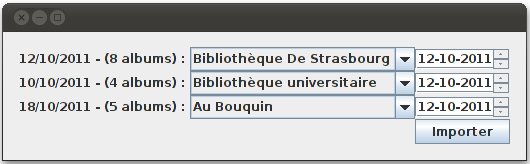
\includegraphics[width=8cm]{img/ajout_import.png}
\end{wrapfigure}
Une fois les emails d'importation sélectionnés, une fenêtre permettant d'entrer le lieu et la date de retour de chaque lots d'emprunts apparaît (un email est égal à un lot).
Le champs de la bibliothèque de cette fenêtre propose, à nouveau, une liste avec les bibliothèques déjà saisies dans l’application.
Ça évite à l’utilisateur de les entrer à nouveau.
La date sera renseignée grâce à un calendrier. La facilité de saisi et d'évitement les erreurs est du coup amélioré. 
Une vérification sur cette date sera aussi mis en place afin de vérifier que cette date n'est pas déjà passée.

Une fois les lieux et dates validés,
une barre de progression affichera l’état de l'importation des lots. 
Une page récapitulatifs des informations ajouté sera affiché une fois l'importation terminé afin de détailler cette importation à l'utilisateur et lui montrer qu'elle à bien fonctionné.
 


\section{Ergonomie dans Royal\_Scanner}
\subsection{Interface graphique}
L'application Royal\_Scanner étant une application pour téléphone Android, il faudra adapter son interface graphique à un affichage mobile ainsi qu'à une utilisation tactile.

\subsubsection{Agencement de la fenêtre}
L’écran d'un téléphone mobile étant plus petit et moins large que celui d'un ordinateur il nous a fallu adapter certains critères d'agencement.

L'application devra veiller à ne pas surcharger l'écran afin que l'utilisation se fasse facilement.

 % \begin{figure}[h!tbp]
  \begin{figure}[h!]
  \begin{center}
    \leavevmode
    \subfloat[Page principal de l'application Royal\_Scanner]{%
		\label{}
		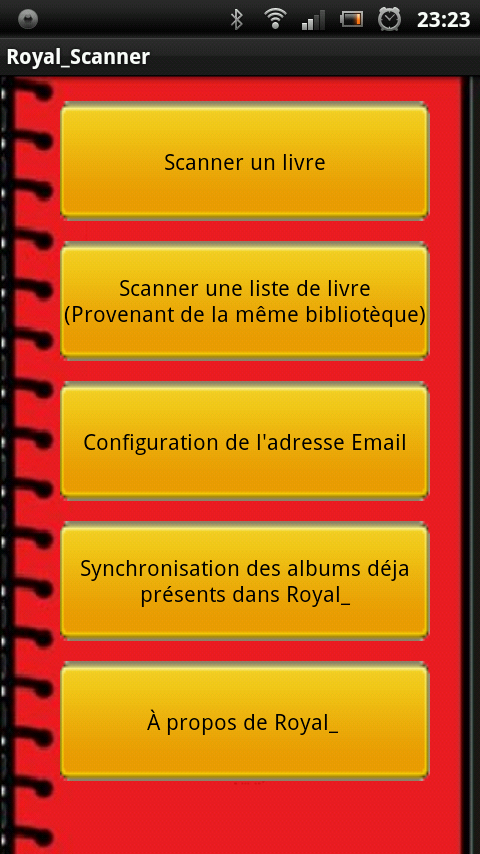
\includegraphics[height=6cm]{img/Menu_Royal_Scanner.png}}
    \hspace{4cm}
    \subfloat[Menu de l'application Royal\_Scanner]{%
		\label{}
		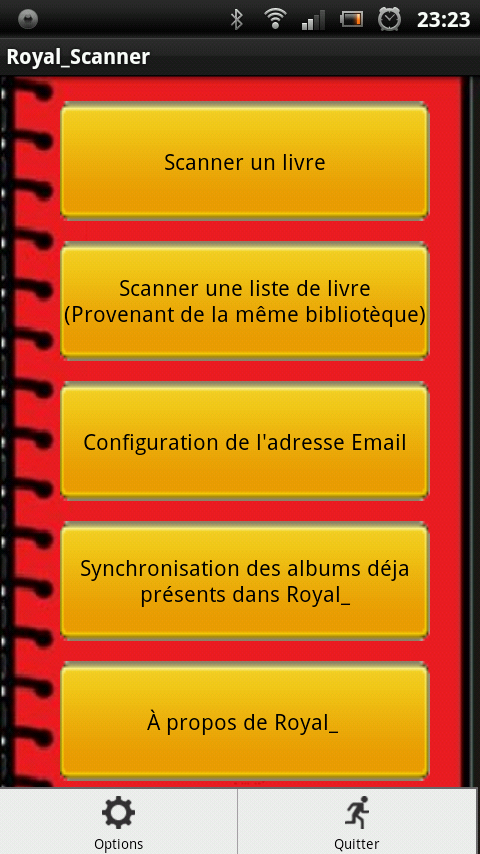
\includegraphics[height=6cm]{img/Menu_Royal_Scanner_option.png}}
  \end{center}
\end{figure}

Afin de proposer les principales actions de l'application mobile à l’utilisateur, une page regroupant les différentes actions sera présenté en guise d'accueil.
Un simple clique sur le bouton de l'action souhaité l'exécutera. 
Afin de garantir leurs accessibilités ces boutons seront assez grand afin d'être adaptés à une utilisation tactile. 

En cas de besoin un menu regroupant les fonctions secondaires sera mis en place.
Ce menu s'ouvrira lors de l’appuie de la touche menu du téléphone. 

  \begin{figure}[h!]
  \begin{center}
    \leavevmode
    \subfloat[Configuration de l'adresse email dans Royal\_Scanner]{%
		\label{}
		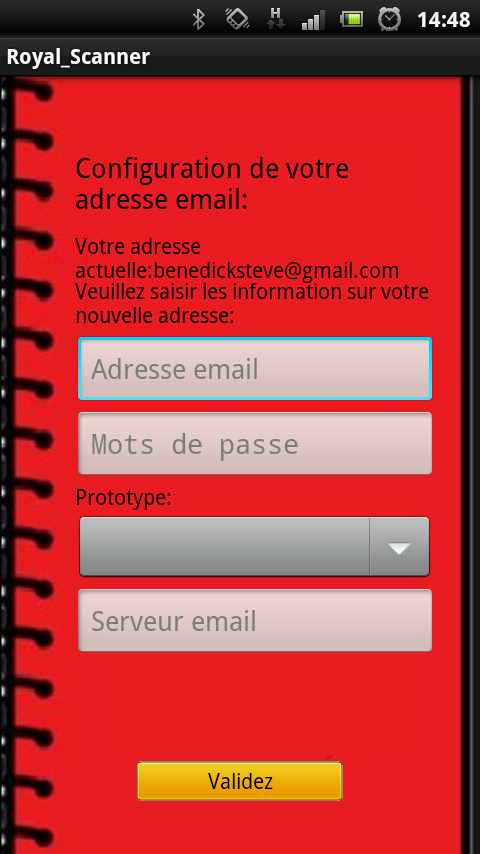
\includegraphics[height=6cm]{img/Configue_Email.png}}
    \hspace{4cm}
    \subfloat[Page d'envoi des ISBN scannés]{%
		\label{}
		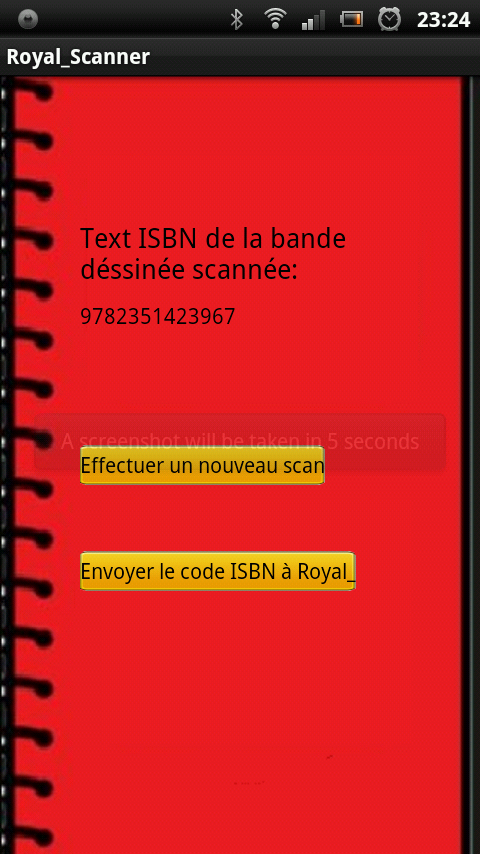
\includegraphics[height=6cm]{img/Scan_Multiple.png}}
  \end{center}
\end{figure}

Dans la page de configuration de l'adresse email le libellé des différents champs sera directement inclue dans le champs lui même.
Ce gain de place permet d'afficher l’intégralité de la page à l'écran ce que nous permet d'éviter l'oublie de champs par l'utilisateur.

Dans la seconde page, correspondant à la page s'affichant après le scan d'un code barre correspondant à un ISBN, le titre du livre sera ajouté à l'ISBN et affiché à l'utilisateur afin de lui montrer le bon fonctionnement du scan. 

\subsubsection{Couleurs et police}
Les couleurs choisies dans l'application \emph{Royal\_Scanner}, bien que rappelant les couleurs du logo de Royal ne sont pas bonnes et devront êtres modifiées.

Des couleurs plus neutres et claires tels que celles utilisées dans l'application PC seront mises en place pour le fond des différentes pages de l’application.

De même la couleurs des boutons sera modifiée en une couleur plus neutre.
Seul le bouton sélectionné aura une couleur plus vive afin d'être distingué des autres. 

Le style d'écriture de l'application \emph{Royal\_Scanner} devrait quand à lui rester le même vu qu'il n'utilise qu'une seule police. 

\subsubsection{Guidage et traitements des erreurs}
Les phases de saisie de l'utilisateur étant moins fréquentes que dans l'application PC nous n'aurons qu'à les gérer dans la configuration de la boite mail.  

Tels que nous l'avons vu précédemment lors de la configuration de la boite email, les libellés de différents champs seront inclus dans le champs lui même.
 
De plus les champs seront configurés selon la valeurs qu'ils doivent retourner afin de proposer à l'utilisateur un clavier tactile optimisé pour la saisie de ces valeurs (par exemples pour le champs de l'adresse email un clavier proposant la touche '@' sera proposé, pour des nombres, un clavier numérique, etc.).

Des vérifications seront aussi effectuées lors de la validation de la boite email sur la validité des différents informations contenues dans les champs.

En cas d'erreurs, un message invitant l'utilisateur à ressaisir certaines informations s'affichera en rouge à l'écran afin d'être vu par l'utilisateur. 

\end{document}
